% Created 2017-03-08 Wed 10:41
% Intended LaTeX compiler: pdflatex
\documentclass[sigconf]{acmart}
\usepackage[utf8]{inputenc}
\usepackage[T1]{fontenc}
\usepackage{graphicx}
\usepackage{grffile}
\usepackage{longtable}
\usepackage{wrapfig}
\usepackage{rotating}
\usepackage[normalem]{ulem}
\usepackage{amsmath}
\usepackage{textcomp}
\usepackage{amssymb}
\usepackage{capt-of}
\usepackage{hyperref}
\usepackage{epigraph}
\author{Nick Merrill, John Chuang}
\affiliation{%
  \institution{BioSENSE, UC Berkeley School of Information}
  \city{Berkeley} 
  \state{California, USA} 
}
\email{ffff@berkeley.edu}

\hypersetup{
 pdfauthor={},
 pdftitle={},
 pdfkeywords={},
 pdfsubject={},
 pdfcreator={Emacs 25.1.1 (Org mode 9.0.4)}, 
 pdflang={English}}

%% I do have one minor revisions I'd like to ask you to make. I found this sentence in the abstract a bit confusing: "I forward a theory of polemic computation, in which the feat of expending material (ecological, labor, and opportunity) costs, rather than particular computational results, exert agency in particular sociotechnical discourses."  Could you revise/clarify? In particular, I was confused by whether "costs" was acting as a noun or verb.

\begin{abstract}
In February of 2017, Google announced the  first SHA1 collision.
Using over nine quintillion computations (over 6,500 years of compute time),
a group of academic and industry researchers produced two different PDF files with identical SHA1 checksums.
But why? After all, SHA1 had already been deprecated by numerous standards and advisory bodies.
This paper uses the SHA1 collision compute as a site for surfacing the space of ecological risks, and sociotechnical rewards, associated with the performance of large computes.
I forward a theory of polemic computation,
in which computes
exert agency in sociotechnical discourses
not through computational results,
but through \textit{feats},
the expenditure of significant material resources.
This paper does not make specific claims about the (ecological, political, labor) limits within which polemic computes must operate in order to be considered acceptable.
Instead, this paper raises the question of how such limits could be established, in the face of polemic computes' significant costs and difficult-to-measure rewards.
\end{abstract}


\begin{CCSXML}
<ccs2012>
<concept>
<concept_id>10010405.10010476</concept_id>
<concept_desc>Applied computing~Computers in other domains</concept_desc>
<concept_significance>500</concept_significance>
</concept>
<concept>
<concept_id>10003120.10003121.10003126</concept_id>
<concept_desc>Human-centered computing~HCI theory, concepts and models</concept_desc>
<concept_significance>300</concept_significance>
</concept>
</ccs2012>
\end{CCSXML}

\ccsdesc[500]{Applied computing~Computers in other domains}
\ccsdesc[300]{Human-centered computing~HCI theory, concepts and models}

% We no longer use \terms command
%\terms{Theory}

\keywords{theory, limits, polemics, charisma}

\setcopyright{rightsretained}
\acmDOI{10.475/123_4}
\acmISBN{123-4567-24-567/08/06}
\acmConference[LIMITS '17]{ACM Limits Workshop}{June 2017}{Santa Barbara, California USA}
\acmYear{2017}
\copyrightyear{2017}
\acmPrice{15.00}
\date{\today}
\title{Better Not to Know\\\medskip
\large Polemic Computation, and Ecological Costs in the SHA1 Collision Compute}
\hypersetup{
 pdfauthor={},
 pdftitle={Better Not to Know},
 pdfkeywords={},
 pdfsubject={},
 pdfcreator={Emacs 25.1.1 (Org mode 9.0.4)}, 
 pdflang={English}}
\begin{document}

\maketitle

\epigraph{I insist on the fact that there is generally no growth but only a luxurious squandering of energy in every form!}{Georges Batailles, \textit{The Accursed Share}}

\section{Introudction}
\label{sec:orgbf0ed32}

From protein folding to the discovery of novel drugs,
some large computes are for the best
\cite{Anderson2004}.
But what about computing ever-increasing digits of pi?
What about finding two PDFs with different content, but identical checksums?
Are such computethis s worth
the ecological costs, and the opportunity costs, compared to other things one could compute?

This paper reads the SHA1 collision compute (Section 2), and the various sociotechnical entanglements that motivated it to be performed (rather than simply discussed) (Section 3),
to motivate a theory of \emph{polemic computation} (Section 4), 
computations that
work primarily to enter into sociotechnical discourses.
In the case of the SHA-1 compute, researchers took on a sizeable monitory and environmental cost
to enforce a point of view among specific stakeholders in the (social, political) economy of SSL certificates.
In so doing, the compute's aims are animated by
larger narratives of authenticity, privacy and security on the internet.

Polemic computes, even important ones, weigh political and social goals against ecological (and other) costs.
This paper aims to begin questions about how polemic computes can and should work within ecological limits.
In other words, I aim to surface questions about the limits of how far computation \emph{should} go to prove our point.
I conclude with how this debate might carry forward in distributed computing, web applications and machine learning (Section 6).

\section{Background}
\label{sec:orgcfb3be1}


Before discussing Google's large compute in depth,
this section gives some background on SHA1, and cryptographic hash functions in general.
Cryptographic hash functions are ``one way'' functions: 
they take some data, and produce some new data, such that the original data cannot be recovered from the new data. The output of the hash function is simply called a \emph{hash}.

SHA1 is one cryptographic hash function, designed by the NSA in the early 1990s.
For some block of any-sized data, SHA1 produces a 40-digit string of characters.
It is used in most version control applications to refer uniquely to files. SHA1 may also be used to check for corrupted files. 
Crucially, as I will discuss in Section 3, SHA1 is also used in security-oriented protocols such as SSH/TLS.


\subsection{SHA1 collisions}
\label{sec:orgd7b902f}

The hashes output by SHA-1 are typically 40 digits, regardless of the size of the input data.
Crucially, hashes \emph{should} relate uniquely to input data: 
two different inputs should never produce the same hash (even though hashes are much smaller than the original data).
A \emph{collision} refers to the breakdown of this property,
in which two different input data produce identical hashes.

Collisions break several common uses of SHA1. 
(Amusingly, a test that captured Google's collision test broke the version control system for the Webkit browser engine \cite{Koivisto2017}).
In the case of SSL/TLS, the protocol for encrypted and authenticated communication on the web, SHA1 collisions have more severe consequences.
Section 5 will return to TLS vulnerability in more detail.

\subsection{SHA1 collisions in theory}
\label{sec:org70172ff}

In discussing the safey of particular hash functions, two questions must be asked:
(1) how long would it take to find a collision by brute force?, and 
(2) is there any algorithm that allows us to find a collision faster than the brute force method?
For the brute force method, the odds of finding a SHA-1 collision by chance are one/2\(^{\text{80}}\)
\cite{Schneier2005}.
In general, the security of this brute-force attack is judged relative to the outer edge of high-end hardware, and hash functions are expected to be retired in time, as computers grow more powerful.
However, this 2\(^{\text{80}}\) space of possibilities in the search for a collision is not considered feasible, so SHA-1 appears safe.

In 2005, however, Wang, Yin \& Yu found an algorithm to produce SHA-1 collisions in under 2\(^{\text{69}}\) calculations (about 2,0000 times faster than the brute force approach)
\cite{Wang2005}.
(It is worth noting that other work had suggested possible weaknesses of SHA-1 earlier \cite{Biham2005}).
While such a compute was, at the time, outside the limits of even powerful adversaries,
the result caused concern among cryptographers \cite{Schneier2005}.
By 2011, a 2\(^{\text{61}}\) calculation attack was discovered \cite{Stevens2013a},
and by the mid 2010s, the developers of most major browsers had announced plans to stop accepting SHA-1 SSL certificates 
\cite{Mozilla2017,Sleevi2014}.


\section{Performing a Collision}
\label{sec:orgb8deeb2}

The study in question here produced two PDFs with different content, but identical SHA-1 hashes
\cite{Stevens2017}.
the study in question performed a SHA collision in 2\(^{\text{63.1}}\) computations, 
and released the source code for replicating the attack
\cite{Stevens2017github}.

Compared to the 2\(^{\text{61}}\) theoretical attack, the practical attack took a bit longer due to the communication overhead required to coordinate computations across several datacenters, and due to the relative inefficiency of using GPUs rather than CPUs.
In practice, the computation required to produce the SHA1 collision required 6,500 years of CPU time and 110 years of GPU time. While this number certainly sounds high, 600,000 cores, each running two threads, could take only two days of compute time.

Of course, time is not the only cost to consider.
Computation is material, physically instiantiated, and has physical, ecological consequences.
Beyond monetary cost, such large computations have very real costs in energy.
Since the implementation details of the infrastructures used for the large collision compute are not entirely knowable from the paper,
it is difficult to estimate this energy cost.
As a rough point of comparison, the monetary cost of such a compute on Cray supercomputers would be on the order of a million dollars
(though such estimates might vary widely in either direction from system to system)
\cite{Pautsch2016}.
In any case, such a figure is a tiny sliver of Alphabet, Inc's over 90 billion dollar revenue in 2016.

This section gave background on SHA1 collisions, 
and gave context for the costs (in time and energy) of the SHA1 collision compute.
The following section details possible explanations for why the computation was performed
in practice, rather than simply discussed in theory.


\section{Explaining why the compute happened}
\label{sec:org911d416}

\begin{figure*}
\centering
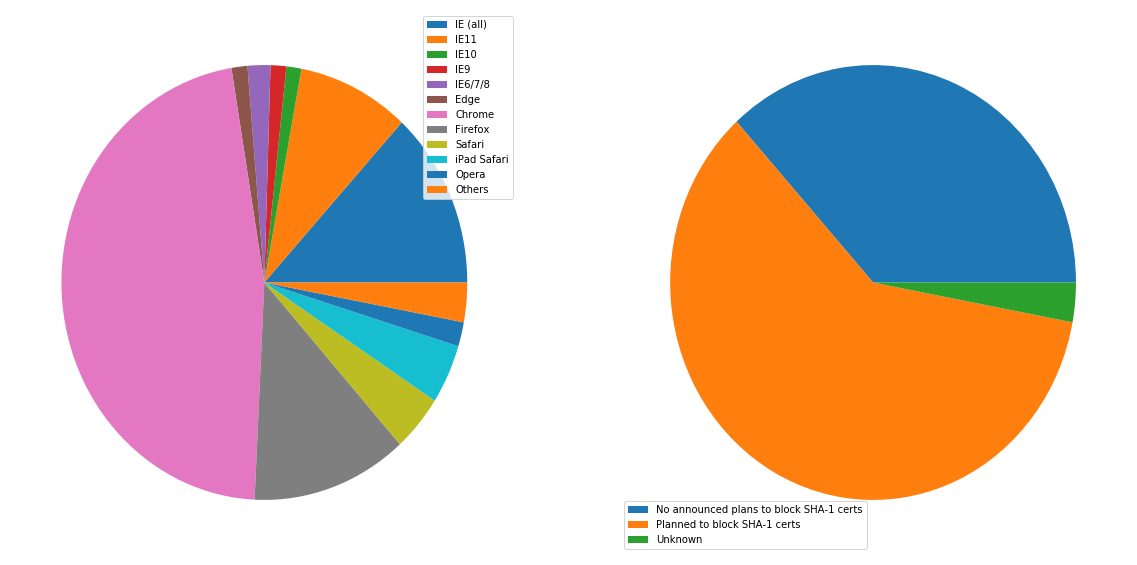
\includegraphics[width=.9\linewidth]{./figures/browser-share.png}
\caption{TODO Explain how many browsers would have ignored SHA-1s anwyway, even if this compute never happened.}
\end{figure*}

Since a theoretical result already existed showing a SHA1 collision was possible, 
one might rightly wonder why researchers would go through a great deal of time and effort
(not to mention a great deal of expense, both monetary and ecological)
to produce artifacts of no practical purpose (different PDFs with identical checksums).
What are the possible benefits?

In this section argues that
the SHA-1 collision compute had essentially polemic goals.
It was performed not to know a particular answer
(as the PDFs themselves are not useful as artifacts), 
but to know that such an answer \emph{has} been found,
as opposed to \emph{can} be found.
I argue that the performance of this collision compute
was necessarily entangled in a particular sociotechnical discourse,
and aimed to change opinions and behavior among specific groups of stakeholders.
This section focuses in particular on those involved in the ecosystem of SSL certificates: browsers, webmasters, and the certificate authorities (CAs) tasked with generating certificates.

\subsection{Practice versus theory}
\label{sec:orga4c40e6}

Before progressing onto a discussion of this compute on the ecosystem of SSL certificates,
we must briefly argue for why an argument of academic interest does not sufficiently explain the performance of this compute.

The computation here ended up being more difficult than theoretical results indicated due to the storage and communication requirements necessary to perform the work across multiple datacenters. 
The collision compute reveals details relevant
to knowing how realistic the threat is in practice. 
Of course, given that SHA1 has already been widely deprecated, this explanation does not in itself answer why such an exercise was considered necessary.
After all, one would not need to know the cost in practice of such an exercise without some reason.

Indeed, one reason, aside from the particular answer computed, is that the compute raises a question and challenge to users of SHA-1:
``Do SHA-1 users have assets worth at least as much as the cost of this compute?''
All cryptography can be broken with sufficient computational time.
This result shows that a powerful attack (such as Google) can indeed break SHA1 with some knowable resources.
And, surely, if Google can perform such an attack, a government actor could do so as well.

Of course, some users of SHA1 did not care much about the demonstrated attack.
Linus Torvalds, developer of the Git version control software (which relies on SHA1 to refer to files), reported no immediate concern.
``Do we want to migrate to another hash? Yes. Is it 'game over' for SHA1 like people want to say? Probably not.'' \cite{Torvalds2017}.
The following section explains the performance of this collision in the context of 
an application in which stakes are potenitally much higher:
the issuance of SSL certificates, some of which rely on SHA-1 to provide cryptographic guarantees.

\subsection{SHA-1 and SSL Certificates}
\label{sec:orge63bf8f}

SHA1 is also used in the issuance of (especially older) SSL certificates.
(SSL certificates
provide a token of the authenticity of a user's connection to a webpage,
and encrypts data end-to-end).
This practical result showed that soembody with the power to perform a SHA1 collision could
now make a fake certificate for a website with that uses SHA1 for nerits TLS.
Such a false certificate could
be used to convince a victim that they are communicating with a given website,
when in fact they are communicating with the attacker.

SSL certificates are issued by Certificate Authorities (CAs), which in theory abide by 
regulations set by the CA/Browser Forum, a standards-setting body.
Here unravels a more complex story of regulation and standards bodies,
as well as stakeholders for whom a change away from SHA-1 could incur significant monetary costs.
The following sections examine the polemic impact of this attack on both CAs, and browser developers. 

\subsubsection{Certificate authorities}
\label{sec:org109f70c}

First, the SHA-1 attack can be mediated entirely by
by replacing old SHA1 certificates with newer ones using SHA-2 or SHA-3.
Second, CAs that abide by CA/Browswer Forum rules are already forbiddedn from issuing SHA-1 certificates. (They are additionally required to insert at least 64 bits of randomness, in an effort to mitigate devistating effects from future cryptographic breaks) \cite{Stevens2017}.

However, Since CAs are decentralized, and since SSL issuees (website administrators) do not routinely check issued SSL certificates for these properties, enforcing these regulations is a perenial challenge for the CA/Browser Forum. It is not clear that CAs were abiding by either of these rules.
Assuming they were not, one explanation for performing this compute is that doing so would encourage CAs (and webmasters) to wisen up to the threat posed by SHA-1,
putting some real pressure on them by freely releasing code that could result in forged certificates \cite{Stevens2017github}.

\uline{quick conclusory paragraph\ldots{}\ldots{}\ldots{}\ldots{}.}

\subsubsection{Browser developers}
\label{sec:orgce90532}

Alongside the issue of enforcing proper security practices on a decentralized system of certificate authorities, 
a separate ecosystem of browser developers exercises independent authority to accept, or reject, certificates issued by CAs.
While browser production is also decentralized, it is less so than CAs (Figure 1).
\url{https://w3techs.com/technologies/overview/ssl\_certificate/all} \uline{pie chart of this graph\ldots{}.next to browser share}

According to these statistics, \uline{the majority??????} of browsers on the web had already agreed to stop accepting SHA-1 SSL certificates,
even before this compute took place
\cite{Sleevi2014,Mozilla2017}.
So, regardless of what certificate authorities do, users of these browsers would have been protected from any vulnerabilities in SHA-1, 
and the CAs would have faced additional market pressure to move away from SHA-1.

If the performance of the collision compute was not necessary to change behaviors among browser developers
(and thus to protect users),
why was it performed?
One explanation may come from the press room.
Browser developers such as Mozilla and Google have gotten flack from their decision to reject SHA-1 certificates,
given the still-theoretical nature of the hash's vulnerability.
\uline{so, another explanation is that this thing helps their PR by bolstering their decision, making it seem more reasonable or wahtever}.
\uline{it will probably stop such back-and-forth all together, helping ppl focus on other issues\ldots{}\ldots{}this alone could have economic impacts within Google, Mozilla}
\uline{at a very high level, browsers need their users to feel secure, or people will not use the web as much!!!!!!}

\subsection{{\bfseries\sffamily TODO} Extravegance, power}
\label{sec:org38ae442}

The SHA-1 collision demonstrated an attack feasible only for highly resourceful actors (for now). 
Such actors might be a government or, apparently, Google.
Thus, this collision demonstrated not only the considerable resources required to exploit \uline{[]}'s theoretical result,
but the vast resources that Google must have, if it is able to spend so heavily on a project with essentially polemic aims.

One explanation is that this computation had the ulterior polemic aim of demonstrating Google's vast resources.
\uline{demonstration of brute strength\ldots{}\ldots{}\ldots{}\ldots{}\ldots{}\ldots{}\ldots{}\ldots{}.and thus power}

\uline{or, alternatively,}
By Bataille's theory of consumption \uline{[]}, some share of all economic activity must be spent without gain 
\uline{1 more sentence here, about extravegance\ldots{}..}.


\section{The polemics of actually doing}
\label{sec:org93057b3}

The prior section gave sociotechnical context for the performance of the SHA-1 collision compute,
giving many explanations across a wide variety of contexts.
However, as of now, we lack a theory for systematically typifying these disparate explanations.
In this section, I propose a definition of \emph{polemic computation} to describe motivations for performing computes such as those above (Section 5.1).
Namely, we propose that some computation is performed because there is a polemic power to doing so, 
and that the material resources expended on such a computation take agency in particular sociotechnical debates.
We tie this theory to that of charismatic technology (Section 5.2)
and to critical design (Section 5.3)
in centering the material nature of performed computation
in describing its agential power in sociotechnical discourses.

\subsection{Defining polemic computation}
\label{sec:org726fca6}

This paper defines \emph{polemic computation} 
as a computation enacted (rather than discussed)
in order to forward an argument or ideology.
Crucially, computations are material artifacts, 
produced in time and energy 
\cite{Dourish2011a}.
Additionally,
their performance or enactment requires 
specialized technical expertise in the form of labor.
Polemic computes are at once feats and artifacts, which act
as an agent in technosocial debates \cite{Ames2015}.

The following sections relate this theory of polemic computations
to other theories of charismatic technology and critical design,
highlighting the relevant differences between our theories and these. 

\subsection{Charismatic technology}
\label{sec:org1bc6f55}

Indeed, polemic computation can be said to ``work'' in part 
because it is animated by ideological frameworks.
In the case of the SHA-1 computation,
ideals that web communications \emph{should} be private and authenticated
very much animate the particular computations that occurred.
These ideals become especially clear when one examines the motivations for actually performing the compute,
even though they were already discussed in theory.

Polemic computation draws srongly to Ames' theory of \emph{charismatic technology}
\cite{Ames2015}.
Drawing on actor-network theory, charismatic technology would ascribe the very artifact of the computation
(a material artifact produced by material means \cite{Dourish2011a,,Bennett2013a})
agency in the technosocial discourses around privacy and security.
Indeed, much like in Ames case of the One Laptop Per Child project,
polemic computation aims to change behavior and beliefs among specific stakeholders in specific debates.

\uline{power, about power indeed power plays in here as the resources are a "feat" for which uch power is required\ldots{}\ldots{}\ldots{}.works in th polemic debate\ldots{}\ldots{}\ldots{}\ldots{}}

However, in contrast to charismatic technology, polemic computation 
centers the material act of computing as a \emph{feat} with costs in time and energy.
In energy, computation expends valuable and scarce ecological resources \cite{SixSilberman2015}.
In time and energy, computational incurs opportunity costs, through answers that could have been computed but were not.
Rather than computing answers, polemic computation uses the material feat of expenditutre
to work as an agent in technosocial discourse.

\subsection{Critical design}
\label{sec:org7ccf681}

Another strand of research that explicitly centers the agency of technological artifacts
is critical design \cite{Dunne2001}.
Critical design seeks to harness the agency of technical artifacts 
to challenge assumptions or surface lurking cultural narratives.
In many ways, polemic computation serves as a critical artifact.
The SHA-1 collision compute, for example, 
called out the poor security practices of many certificate authorities.
Specifically, the material production of the computation,
combined with its almost satirical nature (the compute produced PDFs),
acted to \emph{define} what is and is not a poor security practice for certificate authorities.
Much in the tradition of critical design
used its material power \cite{Bennett2013a} along with a touch of humor to enter into technosocial debates and imaginaries.


\section{Ecological Risks, Polemic Rewards}
\label{sec:orgb3ba397}

The prior section outlined explanations for why the SHA1 compute was performed, 
and proposed a theory of polemic computation typifying such explanations.
A separate question that I have not yet addressed 
is whether or not the compute \emph{should} have been performed,
given the ecological costs (energy and CO2), and the opportunity costs (what else could they could have computed instead, e.g. protein folding). 

More generally, in the case of computations with polemic aims,
how do we decide when to compute?
How can we weigh costs (of all sorts) against the potential (polemic) benefits?
This question could be framed from both an ethical perspective, 
and from an econometric one.

In this section, I outline a few kinds of large compute projects, 
highlighting ways in which they could be considered polemic,
and surfacing the field of risks (and rewards) associated with each.
In general, future work should explore the space of risks and rewards
associated with polemic computes from a variety of ethical, legal and economic standpoints.

\subsection{Volunteer distributed computing projects}
\label{sec:orga3d3a49}

Some projects have aimed to perform large computations by distributing the work across multiple machines,
particularly commodity hardware supplied by volunteers.
A popular platform, BOINC (Berkeley Open Infrastructure for Network Computing)
allows projects to utilize a vast network of volunteers' computing time, 
for example, when their laptop is idle, as a screensaver
\cite{Anderson2004}.
The power of this approach lies in its ability to scale ``horizontally,''
across a wide variety of readily-accessible (and widely deployed) machines.

However, individual machines may not be as efficient in power 
as large-scale server farms.
Additional costs in energy are incurred by added network transmissions,
and the generally lower power-efficiency of commodity devices.
These projects reduce capital overhead for those running the compute,
but may exarcerbate ecological risks.

Future work might examine volunteer computing projects through the lens of polemic computation.
Projects like SETI (Search for Extraterrestrial Intelligence at Home), which have users perform fast fourier transforms on billions of hours of radio recordings,
serve as much to engage in discourses around science and the public as they do to produce useable data 
\cite{Anderson2004}.
The computational work (and associated costs) might be fruitfully examined to other distributed projects, 
such as protein folding.

\subsection{Web applications as supercomputation}
\label{sec:orga08f9a8}

Web applications share some properties with the volunteer distributed computing applications mentioned above.
Much computation is offloaded onto commdity clients, such as mobile phone apps or web browsers.
Consumers of these applications trade their computational time, and electricity, in exchange for the service.
Consider netflix, which retains a centralized system of indexing and content delivery,
but offloads to consumers the processing associated with watching videos 
(downloading videos, along with decrypting the digital rights management, decoding the video format, and finally playing the video and audio).

Future work might exammine the motivations for architectural decisions in web applications through 
the polemics around Web 2.0 
\cite{Scholz2008},
examining how discourse around ``thin clients'' and ``the cloud''
interact with technical constraints
to influence decisions in where processing takes place.
Such polemic decisions may have real ecological consequences.


\subsection{Rise of machine learning}
\label{sec:orgb032e46}

Some work in machine learning blurs the line 
between polemic intent and answer-finding.
Image recognition benchmarks provide one example of this phenomenon:
while a good image recognition algorithm certainly \emph{can} have intrinsic value in other domains 
(e.g, in transfer learning \cite{Jean2016f}),
the production of such an algorithm is often incidental to the production of the benchmark.
Benchmarks serve to mark or legitmize the algorithm's architecture (especially in the case of neural nets)
for the classification problem.

Meanwhile, contemporary machine learning techniques, especially the training of neural nets, 
require a tremendous amount of computation, and therefore a large expenditure of energy.
Thus, when training algorithms in a computationally complex way,
we must ask questions about the costs (and motivations) for doing so.
Future work could raise questions about the polemics involved
with particular attempts to train deep learning algorithms,
examining their ecological costs against the sociotechnical goals 
of performance in particular competitions, or against particular benchmarks \cite{SixSilberman2015}.


\section{Conclusion}
\label{sec:orgeed12ab}

Using the example of a relatively modest large-scale compute,
this paper highlights broader tensions about when and when not to compute.
In the case of polemic computation, the social rewards are always unclear.
Future work should consider broadly what we can we do to hedge our risks, 
not just in time and captial,
but in ecological cost.
We will only have more things to compute,
and more things to compute them with,
but how to select which to expend our increasingly precious resources on, 
how to use restraint?


\section{Acknowledgements}
\label{sec:org85cf661}
Morgan Aimes, Nick Doty, Anette Greiner, Sebastian Benthall

\bibliographystyle{ACM-Reference-Format}
\bibliography{refs}
\end{document}
